Usability is a \emph{`quality attribute that assesses how easy interfaces are to
    use'} (\cite{usabilitycomponentsnielsen}). The best way to assess the usability
of an interface is to conduct usability testing.

Also referred to as \emph{user testing} is a popular UX research methodology
used to uncover problems in the user interface design of an application and
learn about the target user's preferences (\cite{usertestingdefinition}).

\noindent There are 3 core elements to user testing: \textbf{the facilitator},
\textbf{the participant} and \textbf{the tasks}. The facilitator administers the
tasks to the participant, observes their behaviour and listens to their
feedback.

\noindent Our approach is as follows:
%user evaluation process
\begin{figure}[h!]
    \centering
    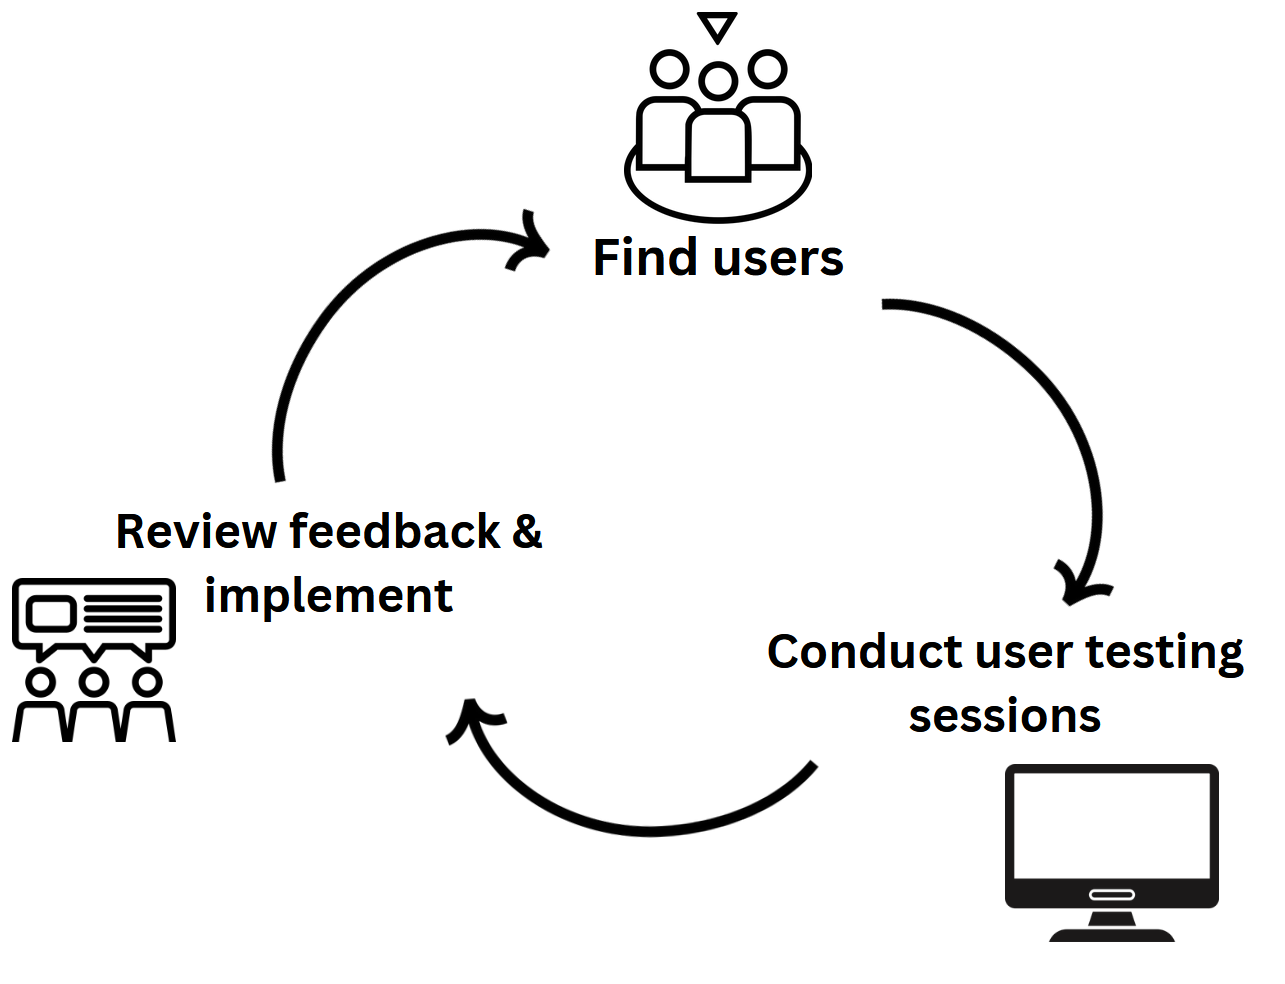
\includegraphics[width=0.6\textwidth]{images/user-eval-process.png}
    \caption{User Evaluation Process}
\end{figure}

Firstly, users from the research survey who left their contact were recruited to
participate in user testing. Additionally, a call for participation was made
through social media channels to seek out other users.

Next, online user testing sessions were conducted to discuss Magpie, explore the
features and gather feedback. The notes taken during the sessions were then
synthesized and reviewed to gather a list of new features to implement, items to
change and content to remove. Lastly, the process started again in order to continue
improving Magpie's workflow and interface.

There were 11 in-depth interviews in total, that have been divided into the
following categories: 6 Non-Expert Users, 3 Domain Expert, 1 UI/UX expert and 1
accessibility expert.
\emph{Non-Expert Users} are defined as those who use Magpie casually for personal
interests.
\emph{Domain Experts} are defined as those who use Magpie as a tool
for their work.

It is worth nothing that some users have decided to remain anonymous, therefore have
been labelled as \emph{Anonymous n°}, while others will be referred to by their
name.

\newpage{}

\noindent Both controlled \& uncontrolled approaches were used for the sessions.
The controlled sessions were based around a strict list of tasks the user would
complete and used metrics such as time taken, difficulty and task success rate.
The uncontrolled sessions let the users freely roam the application while we
observed their behaviour interacting with each element and initiate discussion
to obtain feedback on features to improve.

\noindent A table with a list of general tasks is used to quantitatively
evaluate each feature the user interacted with. Metrics measured are task
difficulty and task success rate. The list of general tasks increased as the
test sessions went on because new features were being added iteratively.

The difficulty of the task is related to its status and how much time a user
spent on it. The status of a task can either be \emph{`complete'},
\emph{`pass'}, or \emph{`fail'} where:

\begin{itemize}
    \item \emph{complete} is attributed when the user completes the task on
          their own. This is worth 1 point.
    \item \emph{pass} is attributed when the user was able to complete the task
          but with our help. This is worth 0.5 points.
    \item \emph{fail} is attributed when the user was not able to complete the
          task even with our help. This is worth 0 points.
\end{itemize}

Lastly, a short satisfaction survey in Figure \ref{fig:userevalquestions} is
administered at the end of each session to quantify user experience and provide
a baseline for improvements. User behaviour is also observed during the session
to complement these quantitative metrics.

The evaluation of Magpie has been divided into the following sections:
\begin{enumerate}
    \item Non-Expert Users test sessions
    \item Domain Experts test sessions
    \item UX/UI expert review
    \item Accessibility expert review
\end{enumerate}
